\section{Shortest Paths}\label{sec:1}

\subsection{Preliminaries on Graphs}\label{subsec:1.1}
An {\bf (undirected) graph} $G$ is a pair $(V, E)$, where $E$ is a set of 
unordered pairs of elements in $V$. The elements of $V$ are called {\bf vertices}
or {\bf nodes}; the elements of $E$ are called {\bf edges}. 

Let $u, v \in V$ and let $e = uv \in E$ be an edge. 
\begin{itemize}
    \item We say that $e$ is {\bf incident} to $u$ and $v$. 
    \item The vertices $u$ and $v$ are said to be {\bf adjacent}.
    \item We call $u$ and $v$ the {\bf endpoints} of $e$. 
\end{itemize}
By default, we assume that there are no parallel edges (i.e. two
edges $e = uv$ and $e' = u'v'$ in $E$ with $\{u, v\} = \{u', v'\}$) 
and no loops (i.e. an edge $e = uv \in E$ with $u = v$).

For distinct $u, v \in V$, a {\bf $u, v$-path} is a sequence of vertices 
$w_1, \dots, w_k$ such that $w_1 = u$, $w_k = v$, and $w_i w_{i+1} \in E$ 
for all $i = 1, \dots, k-1$.  

For example, consider the following graph $G = (V, E)$ with 
vertices $V = \{v_1, v_2, v_3, v_4\}$ and edges $E = \{v_1v_2, v_1v_4, v_2v_3, 
v_2v_4, v_3v_4\}$. 

\begin{center}
    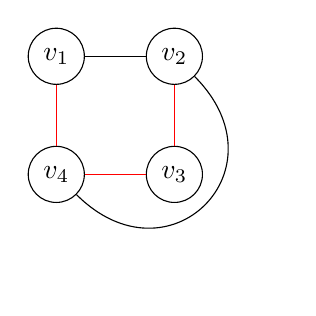
\begin{tikzpicture}[node distance={15mm}, main/.style = {draw, circle}] 
        \node[main] (1) {$v_1$}; 
        \node[main] (2) [right of=1] {$v_2$};
        \node[main] (3) [below of=2] {$v_3$}; 
        \node[main] (4) [left of=3] {$v_4$};

        \draw (1) -- (2);
        \draw [draw=red] (1) -- (4);
        \draw [draw=red] (2) -- (3);
        \draw (2) to [out=315, in=315, looseness=2] (4);
        \draw [draw=red] (3) -- (4);
    \end{tikzpicture} 
\end{center}
\vspace{-0.5cm}

The lines in red form a $v_1, v_2$-path, namely $v_1, v_4, v_3, v_2$. 
Another $v_1, v_2$-path can be obtained by simply traversing the edge $v_1v_2$. 

A {\bf cycle} in $G$ is a sequence of vertices $w_1, \dots, w_{k+1}$ 
such that $w_i w_{i+1} \in E$ for all $i = 1, \dots, k$, the vertices 
$w_1, \dots, w_k$ are all distinct, and $w_1 = w_{k+1}$.

Finally, a graph $G$ is {\bf connected} if for any pair of distinct vertices 
$u, v \in V$, there exists a $u, v$-path in $G$. 

\subsection{Shortest Paths Problem}\label{subsec:1.2}
Given a \emph{directed} graph $G = (V, E)$ with edge lengths $\ell_e \geq 0$
for each $e \in E$ and a distinguished start vertex $s \in V$, we wish 
to find shortest paths from $s$ to every other vertex in $V$. Note that 
when we work with directed graphs, we will denote the directed edges 
with $(v_1, v_2)$ as opposed to $v_1 v_2$ in the case of undirected graphs, where 
the order of the vertices did not matter. 

The {\bf length} of a path $P$ given by the sequence $w_1, \dots, w_k$ 
is given by 
\[ \ell(P) := \sum_{i=1}^{k-1} \ell_{(w_i, w_{i+1})} = \sum_{e\in P} \ell_e, \] 
where the second sum makes sense because there are no parallel edges. 
Then the {\bf shortest-path distance} from $s$ to a vertex $u \in V$ is 
defined to be
\[ d(u) := \min_{\text{$s,u$-paths $P$}} \ell(P). \] 
For example, we can consider the following instance of an undirected graph 
with given edge lengths and starting vertex $s = v_1$. 

\begin{center}
    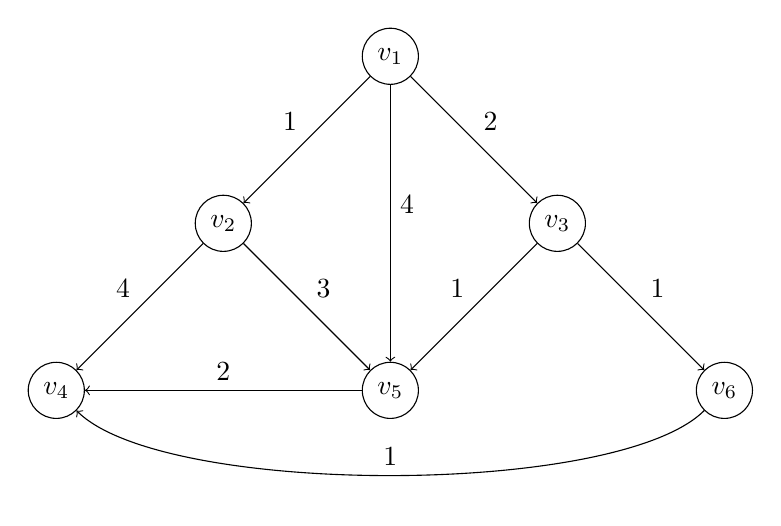
\begin{tikzpicture}[node distance={30mm}, main/.style = {draw, circle}] 
        \node[main] (1) {$v_1$}; 
        \node[main] (2) [below left of=1] {$v_2$};
        \node[main] (3) [below right of=1] {$v_3$}; 
        \node[main] (4) [below left of=2] {$v_4$};
        \node[main] (5) [below left of=3] {$v_5$};
        \node[main] (6) [below right of=3] {$v_6$};

        \draw[->] (1) -- node[midway, above left] {1} (2);
        \draw[->] (1) -- node[midway, above right] {2} (3);
        \draw[->] (1) -- node[midway, above right] {4} (5);
        \draw[->] (2) -- node[midway, above left] {4} (4);
        \draw[->] (2) -- node[midway, above right] {3} (5);
        \draw[->] (3) -- node[midway, above left] {1} (5);
        \draw[->] (3) -- node[midway, above right] {1} (6);
        \draw[->] (5) -- node[midway, above] {2} (4);
        \draw[->] (6) to [out=225, in=315, looseness=0.5] node[midway, above] {1} (4);
    \end{tikzpicture} 
\end{center}
\vspace{-0.5cm}
In this case, we have $d(v_2) = 1$, since the only possible path from 
$v_1$ to $v_2$ is by taking the edge $(v_1, v_2)$. There are multiple
paths from $v_1$ to $v_5$; the shortest one is $v_1, v_3, v_5$ giving 
$d(v_5) = 3$. 

Note that we always set $d(s) = 0$. We now make some observations: 
\begin{enumerate}[(i)]
    \item If $(u, v) \in E$, then $d(v) \leq d(u) + \ell_{(u,v)}$, since 
    such an $s, v$-path is always an option.
    \item For every $v \in V$ distinct from $s$, there exists $w \in V$ 
    such that $d(v) = d(w) + \ell_{(w, v)}$ and $(w, v) \in E$. This can 
    be seen by chopping off the last edge from a shortest path from $s$ to $v$.
\end{enumerate}

\subsection{Dijkstra's Algorithm}\label{subsec:1.3}
In 1959, Dijkstra came up with the following algorithm to solve the 
shortest paths problem. The main idea is to maintain a set $A \subseteq V$ 
of "explored" nodes; that is, a set of nodes for which we already know the 
shortest-path distances. We'll also maintain labels $d'(v)$ for $v \in 
V \setminus A$ with upper bounds on the shortest-path distances from $s$. 

{\bf Input.} A directed graph $G = (V, E)$, edge lengths $\ell_e \geq 0$ for 
all $e \in E$, and a start vertex $v \in V$. 

{\bf Output.} For all $v \in V$, the length $d(v)$ for the shortest-path from 
$s$ to $v$.
\begin{enumerate}[leftmargin=1.75cm, label={Step \arabic*.}]
    \item {\bf Initialization.} $A \gets \{s\}$, $d(s) \gets 0$, and $d'(v) \gets \infty$ 
    for all $v \in V \setminus A$.

    \item While $A \neq V$:
    \begin{enumerate}[label={Step 2.\arabic*.}]
        \item {\bf Push down the upper bounds.} For each $v \in V \setminus A$, compute 
        \[ d'(v) \gets \min\left\{ d'(v), \min_{\substack{u\in A \\ (u, v) \in E}} 
        \{ d(u) + \ell_{(u, v)} \} \right\}. \] 
        \item {\bf Add a new vertex.} Set $w \gets \argmin_{v \in V \setminus A} d'(v)$, 
        $A \gets A \cup \{w\}$, and $d(w) \gets d'(w)$. 
    \end{enumerate}
\end{enumerate}

Suppose that for each vertex $w \in V$, we keep track of the node $u$ 
determining its upper bound $d'(w)$. That is, the node $u$ is such that 
$(u, w) \in E$ and $d'(w) = d(u) + \ell_{(u, w)}$. Then at the end of the 
algorithm, a shortest path from $s$ to $w$ can be obtained as a shortest path 
from $s$ to $u$ adjoined with the edge $(u, w) \in E$. Moreover, these edges 
selected by Dijkstra's algorithm form an arborescence, which is a nice graph 
structure that we'll discuss more later. 

Next, let's prove the correctness of Dijkstra's algorithm. In particular, 
we need to show that for every $v \in V$, the distance from $s$ to $v$ 
is computed correctly. We'll assume that the graph is connected; that is, 
for every $v \in V$, there is an $s, v$-path in $G$. (Note that the 
algorithm won't terminate otherwise, but it can be adjusted to deal 
with this.)

\begin{pf}[correctness of Dijkstra's algorithm]
    We proceed by induction on $|A|$, and show that at each point in time, 
    $d(v)$ is computed correctly for all $v \in A$. The case where $|A| = 1$ 
    is clear because at the start of the algorithm, we initialize $A = \{s\}$ 
    with $d(s) = 0$, which is correct. 

    Assume that $d(v)$ is computed correctly for every $v \in A$ when 
    that $|A| = k$. Suppose that we are adding a new vertex $w$ to $A$ 
    in Step 2.2 of the algorithm. Consider the vertex $u \in A$ such that 
    $(u, w) \in E$ and 
    \[ d'(w) = d(u) + \ell_{(u, w)}. \] 
    Specifically, this is the vertex $u$ determining the upper bound 
    $d'(w)$ which we discussed in the paragraph following the description 
    of the algorithm. 

    For the sake of contradiction, assume that the distance from $s$ to $w$ 
    is not $d'(w)$. Let $P_u$ be a shortest path from $s$ to $u$, and 
    let $P'$ be a shortest path from $s$ to $w$. Then by our 
    assumption, we know that 
    \[ \ell(P') < \ell(P_u) + \ell_{(u, w)} = d'(w). \] 
    Now, let $x, y \in V$ be such that $(x, y) \in E$ lies on the shortest 
    path $P'$ from $s$ to $w$, with $x \in A$ and $y \in V \setminus A$. 
    (This exists because at some point, the path must exit $A$ to get 
    from $s$ to $w$.) Then we obtain 
    \[ d'(y) \leq d(x) + \ell_{(x,y)} \leq \ell(P') < \ell(P_u) 
    + \ell_{(u, w)} = d'(w), \] 
    where the first inequality is because of how $d'(y)$ is computed in 
    Step 2.1, and the second inequality is because the shortest path 
    from $x$ to $y$ adjoined with the edge $(x, y)$ is part of the path $P'$, 
    noting that $\ell_e \geq 0$ for all $e \in E$. But this contradicts 
    our choice of $w = \argmin_{v\in V \setminus A} \{d'(v)\}$ in Step 2.2 
    since $y \in V \setminus A$ but $d'(y) < d'(w)$. \qed
\end{pf}